% !TeX spellcheck = fa_FA
% !TEX TS-program = xelatex
% !TEX encoding = UTF-8 Unicode

\documentclass[xcolor=dvipsnames, professionalfonts, 11pt]{beamer}
\usepackage{tikz}
\usepackage{xcolor}
\usepackage{xepersian}
\usepackage{euler}
\usepackage{amsmath, amssymb}

% Paper information
\usepackage{xparse}
\NewDocumentCommand{\information}{o g g}{%
\author[]{#2%
\IfValueT{#3}{\vspace{5mm}\\#3}%
\IfValueT{#1}{\vspace{5mm}\\\color{mygray}{\footnotesize \lr{Available at \url{#1}}}}%
}\date[]{}}

% --- Commands ---
\newcommand*{\makeframetitle}{\frametitle{\insertsection \hspace{0.1em} {\footnotesize [\insertsubsection]}}}

% --- Fonts ---
\usefonttheme{professionalfonts} 
\usefonttheme{serif}
\usepackage{fontspec}
\settextfont{main_font.ttf}

% --- Beamer Theme ---
\usetheme{Boadilla}
\usecolortheme[]{seagull}
\setbeamercovered{transparent}
\setbeamertemplate{navigation symbols}{}
\setbeamertemplate{footline}[frame number]

% --- Font sizes and shapes ---
\setbeamerfont{title}{size=\huge, series=\scshape}
\setbeamerfont{author}{size=\large}
\setbeamerfont{frametitle}{series=\scshape}
\setbeamertemplate{frametitle}{\MakeLowercase{\insertframetitle}}
\setbeamertemplate{frametitle continuation}{[\insertcontinuationcount]}
\setbeamerfont{itemize/enumerate subbody}{size=\normalsize}
\setbeamerfont{button}{size=\footnotesize}

% --- Spacing ---
\usepackage[onehalfspacing]{setspace}
\setbeamertemplate{title page}[default][right,rightskip=-8pt]
\addtobeamertemplate{frametitle}{\vskip3mm}{}
\setbeamersize{text margin right=5mm,text margin left=5mm}

% --- Color ---
\colorlet{myblack}{black!85!}
\colorlet{mygray}{gray!60!}
\setbeamercolor{title}{fg=myblack}
\setbeamercolor{frametitle}{fg=myblack}
\setbeamercolor{normal text}{fg=myblack}
\setbeamercolor{itemize item}{fg=mygray}
\setbeamercolor{itemize subitem}{fg=mygray} 
\setbeamercolor{enumerate item}{fg=mygray} 
\setbeamercolor{enumerate subitem}{fg=mygray}
\setbeamercolor{footline}{fg=mygray}
\setbeamercolor{button}{fg=mygray, bg=white}

% --- Lists ---
\setbeamertemplate{itemize item}{\textbullet}
\setbeamertemplate{itemize subitem}{\textendash} 
\setbeamertemplate{enumerate item}[default]
\setbeamertemplate{enumerate subitem}[default]
\setbeamertemplate{enumerate subitem}{\alph{enumii}.}

% % Title capitalization and underline
\let\oldtitle\title
\renewcommand{\title}[1]{\oldtitle[]{\MakeLowercase{#1}\vspace{-2mm}\\\color{myblack}{\rule{\textwidth}{2pt}}\vspace{1cm}}}

% --- Main ---
\author{سید محمد رضا هدایی}
\institute{}

\begin{document}
\title{پیاده سازی رمزنگاری تصویر توسط تابع فرا آشوب 7 بعدی و ماتریس پاسکال}
\information
[https://github.com/smrhodaee/image_encryption]%
{نویسنده : سید محمد رضا هدایی \\ استاد راهنما : دکتر ابراهیم زارعی}%
{دانشگاه اصفهان پردیس خوانسار -- 1402/11/01}
\frame{\titlepage}

\begin{frame}
    \frametitle{فهرست مطالب}
    \only<1>{\tableofcontents[sections={1-4}]}
    \only<2>{\tableofcontents[sections={5-}]}
\end{frame}

\section{مقدمه}
\subsection{چرا به رمزنگاری تصویر نیاز داریم؟}
\begin{frame}
    \makeframetitle
    \begin{itemize}
        \item {افزایش حملات سایبری مخرب}
        \item{محافظت از تصاویر پزشکی و نظامی}
        \item{بهترین نوع میان روش های محافظت از تصاویر}
        \begin{itemize}
            \item \lr{Image WaterMarking}
            \item \lr{Image Steganography}
            \item \lr{\textbf{Image Encryption}}
        \end{itemize}
        \item تبدیل تصویر اولیه به تصویر ناخوانا
    \end{itemize}
\end{frame}

\subsection{چرا از تابع فرا آشوب 7 بعدی استفاده می کنیم؟}
\begin{frame}
    \makeframetitle
    \begin{itemize}
        \item رفع محدودیت های توابع با ابعاد کمتر
        \item غیرخطی بودن
        \item تصادفی بودن
        \item غیر قابل پیش بینی بودن
        \item ساخت دنباله کلید با فضای کلید بزرگ
        \item افزایش سطح امنیت با فرا آشوب بودن
      \end{itemize}
\end{frame}

\subsection{چرا الگوریتم جدید پیاده سازی کردیم؟}
\begin{frame}
    \makeframetitle
    \begin{itemize}
      \item فضای کلید کوچک در الگوریتم های قبلی (حملات بروت فروس)
      \item ناکارایی در حملات نویز نمک فلفلی
      \item امنیت پایین در حملات دیفرانسیلی و آماری
      \item حذف کردن هم بستگی میان پیکسل های همجوار
      \item افزایش تصادفی بودن و غیرقابل پیش بینی بودن
      \item کاهش زمان پردازش
    \end{itemize}
\end{frame}

\section{پیش نیاز ها}
\subsection{ماتریس متقارن پاسکال}
\begin{frame}[allowframebreaks]
    \makeframetitle
    \begin{itemize}
        \item ماتریس مربعی \lr{P(n)} را با ابعاد \lr{n × n} در نظر می گیریم
            \begin{align}
                P_{i,j} = \binom{i + j}{i} = \frac{(i + j)!}{i!j!}, 0 \leq i, j < n.
            \end{align}
            \begin{align}
                p_{i,j} = p_{i-1,j} + p_{i,j-1}
            \end{align}
            \framebreak
            {\scriptsize
            \begin{align}
                P(1) = \begin{bmatrix}
                    1
                \end{bmatrix},
                P(2) = \begin{bmatrix}
                    1 & 1\\
                    1 & 2
                \end{bmatrix},
                P(3) = \begin{bmatrix}
                    1 & 1 & 1\\
                    1 & 2 & 3\\
                    1 & 3 & 6
                \end{bmatrix},
                P(4) = \begin{bmatrix}
                    1 & 1 & 1 & 1\\
                    1 & 2 & 3 & 4\\
                    1 & 3 & 6 & 10\\
                    1 & 4 & 10 & 20
                \end{bmatrix}
            \end{align}
            }
            \item  ماتریس پاسکال معکوس با ابعاد 4*4
            \begin{align}
                P^{-1}(4) = \begin{bmatrix}
                    4 & -6 & 4 & -1\\
                    -6 & 14 & -11 & 3\\
                    4 & -11 & 10 & -3\\
                    -1 & 3 & -3 & 1
                \end{bmatrix}
            \end{align}
    \end{itemize}
\end{frame}

\subsection{سیستم فرا آشوب 7 بعدی}
\begin{frame}
    \makeframetitle
    \begin{align}
        \begin{split}
            \dot{x_1} = -ax_1 + ax_5 - bx_5x_6x_7\\
            \dot{x_2} = -cx_2 + dx_6 + x_1x_6x_7\\
            \dot{x_3} = -ax_3 + ax_5 - gx_1x_2x_7\\
            \dot{x_4} = -ax_4 + ex_1 + x_1x_2x_3\\
            \dot{x_5} = -ax_5 + ex_7 - x_2x_3x_4\\
            \dot{x_6} = -ex_6 + ex_5 + x_3x_4x_5\\
            \dot{x_7} = -bx_7 + fx_2 - hx_4x_5x
        \end{split}
    \end{align}
    \lr{a = 15, b = 5, c = 0.5, d = 25, e = 10, f = 4, g = 0.1, h = 1.5}
\end{frame}
\section{الگوریتم پیشنهادی}
\subsection{الگوریتم رمزنگاری}
\begin{frame}[allowframebreaks]
\makeframetitle
\begin{enumerate}
    \item وارد کردن تصویر خاکستری به عنوان \lr{G}
    \item تبدیل \lr{G} به بردار \lr{V}
    \item محاسبه مقادیر اولیه کلید سیستم فرا آشوب
    \begin{align}
        x_1 = \frac{\sum_{i=1}^{MN} V(i) + MN}{2^23 + MN}\\
        x_i = mod(10^7x_{i-1}), i = 2,3,4,5,6,7
    \end{align}
    \item ساختن دنباله \lr{S} با پیمایش سیستم فرا آشوب 7 بعدی و انتخاب دنباله $$(x_1, x_2, x_7)$$
    \item مرتب کردن \lr{S} به صورت صعودی و برگرداندن موقعیت پیکسل های مرتب شده در بردار \lr{SS}
    \item محاسبه بردار جایگشت داده شده \lr{B} $$ B = V(SS) $$
    \item بردار \lr{B} را به ماتریس \lr{D} با اندازه \lr{MN} تغییر شکل دادن.
    \item ماتریس \lr{D} را به زیرماتریس های مرتبه 4 تقسیم کردن
    \item ماتریس \lr{E} را با ضرب هر زیرماتریس در ماتریس پاسکال مرتبه 4 بدست  آوردن به شکل زیر
    {\footnotesize
    \begin{align}
        \begin{split}
           \begin{bmatrix}
                E_{i,j} & E_{i,j+1} & E_{i,j+2} & E_{i,j+3}\\
                E_{i+1,j} & E_{i+1,j+1} & E_{i+1,j+2} & E_{i+1,j+3}\\
                E_{i+2,j} & E_{i+2,j+1} & E_{i+2,j+2} & E_{i+2,j+3}\\
                E_{i+3,j} & E_{i+3,j+1} & E_{i+3,j+2} & E_{i+3,j+3}
            \end{bmatrix}\\ = 
            \begin{bmatrix}
                D_{i,j} & D_{i,j+1} & D_{i,j+2} & D_{i,j+3}\\
                D_{i+1,j} & D_{i+1,j+1} & D_{i+1,j+2} & D_{i+1,j+3}\\
                D_{i+2,j} & D_{i+2,j+1} & D_{i+2,j+2} & D_{i+2,j+3}\\
                D_{i+3,j} & D_{i+3,j+1} & D_{i+3,j+2} & D_{i+3,j+3}
            \end{bmatrix}
            \begin{bmatrix}
                1 & 1 & 1 & 1\\
                1 & 2 & 3 & 4\\
                1 & 3 & 6 & 10\\
                1 & 4 & 10 & 20
            \end{bmatrix} mod 256
        \end{split}
    \end{align}
    }
    \item با استفاده از دو مرحله از فرآیند رمزگذاری, تصویر رمزگذاری شده \lr{E} را بدست آوردن. به منظور دستیابی به نتایج رمزگذاری بهتر, تنها دو دور فرآیند درهمسازی و انتشار برای اصلاح موقعیت ها و حذف همبستگی بین پیکسل های همسایه در تصویر رمزگذاری شده کافی است.
\end{enumerate}
\end{frame}

\subsection{الگوریتم رمزگشایی}
\begin{frame}[allowframebreaks]
\makeframetitle
\begin{enumerate}
    \item تصویر رمز شده \lr{E} به زیر ماتریس های مرتبه 4 تقسیم می شود و سپس با ضرب هر زیر ماتریس در معکوس ماتریس پاسکال از معادله زیر برای زیر ماتریس های تصویر استفاده می شود.
    {\footnotesize
    \begin{align}
        \begin{split}
            \begin{bmatrix}
                D_{i,j} & D_{i,j+1} & D_{i,j+2} & D_{i,j+3}\\
                D_{i+1,j} & D_{i+1,j+1} & D_{i+1,j+2} & D_{i+1,j+3}\\
                D_{i+2,j} & D_{i+2,j+1} & D_{i+2,j+2} & D_{i+2,j+3}\\
                D_{i+3,j} & D_{i+3,j+1} & D_{i+3,j+2} & D_{i+3,j+3}
            \end{bmatrix}\\ = 
            \begin{bmatrix}
                E_{i,j} & E_{i,j+1} & E_{i,j+2} & E_{i,j+3}\\
                E_{i+1,j} & E_{i+1,j+1} & E_{i+1,j+2} & E_{i+1,j+3}\\
                E_{i+2,j} & E_{i+2,j+1} & E_{i+2,j+2} & E_{i+2,j+3}\\
                E_{i+3,j} & E_{i+3,j+1} & E_{i+3,j+2} & E_{i+3,j+3}
            \end{bmatrix}
            \begin{bmatrix}
                4 & -6 & 4 & -1\\
                -6 & 14 & -11 & 3\\
                4 & -11 & 10 & -3\\
                -1 & 3 & -3 & 1
            \end{bmatrix} mod 256
        \end{split}
    \end{align}
    }
    \item تصویر \lr{D} به دست آمده از فاز قبلی به بردار \lr{U} تبدیل می شود.
    \item محاسبه زیر از بردار \lr{S} ایجاد شده در مرحله رمزگذاری برای بازگرداندن پیکسل ها به موقعیت اصلی خود استفاده می کند:
    \begin{align}
        O(S_k) = U_k; k = 1 : MN 
    \end{align}
    \item بردار \lr{O} را به ماتریس تبدیل کنید تا به تصویر رمزگشایی شده \lr{G'} برسید
    \item برای دستیابی به تصویر رمزگشایی شده, دو بار فرآیند رمزگشایی مورد نیاز است
\end{enumerate}
\end{frame}

\section{نتایج شبیه سازی}
\subsection{پلت فرم آزمایش}
\begin{frame}
    \makeframetitle
    برای نشان دادن توانایی اگوریتم های رمزنگاری و رمزگشایی پیشنهادشده از یک لب تاب با پردازنده اینتل \lr{core i5} و با حافظه \lr{12 GB} استفاده می کنیم هم چنین الگوریتم توسط پایتون پیاده سازی شده است
\end{frame}

\subsection{نتایج آزمایش}
\begin{frame}[allowframebreaks]
    \makeframetitle
    کارایی الگوریتم را با تصاویر مختلف مورد ارزیابی قرار میدهیم
    که به شکل ریز می باشد (به ترتیب \lr{Tank 256*256} , \lr{Boat 512*512}, \lr{Lena 512*512}, \lr{Cameraman 1024*1024}, \lr{CTScan 1024*1024})
    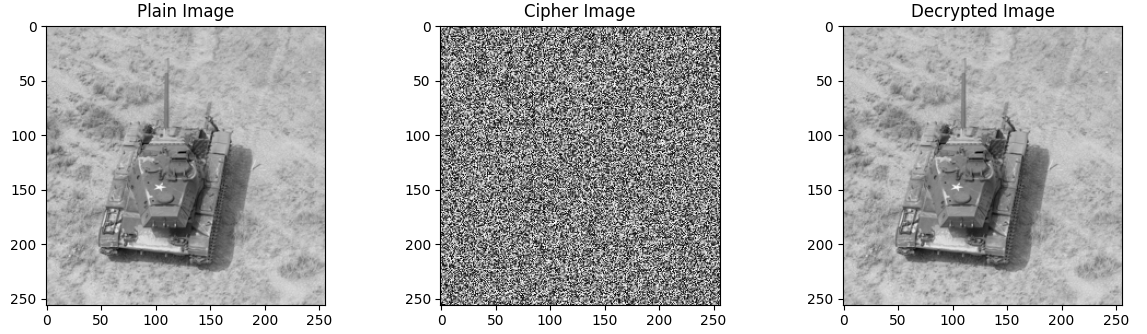
\includegraphics[width=\textwidth]{assets/result01.png}
    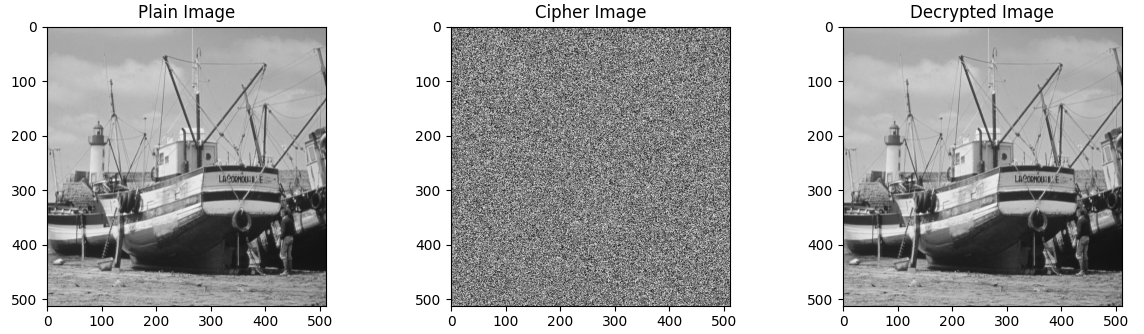
\includegraphics[width=\textwidth]{assets/result02.png}
    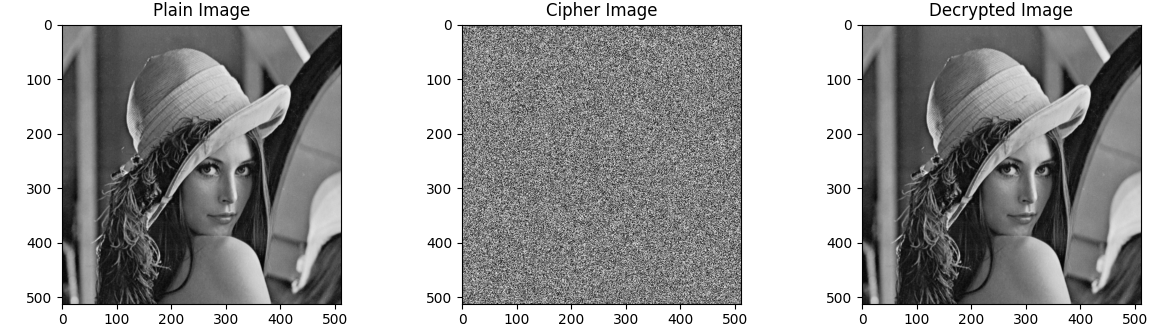
\includegraphics[width=\textwidth]{assets/result03.png}
    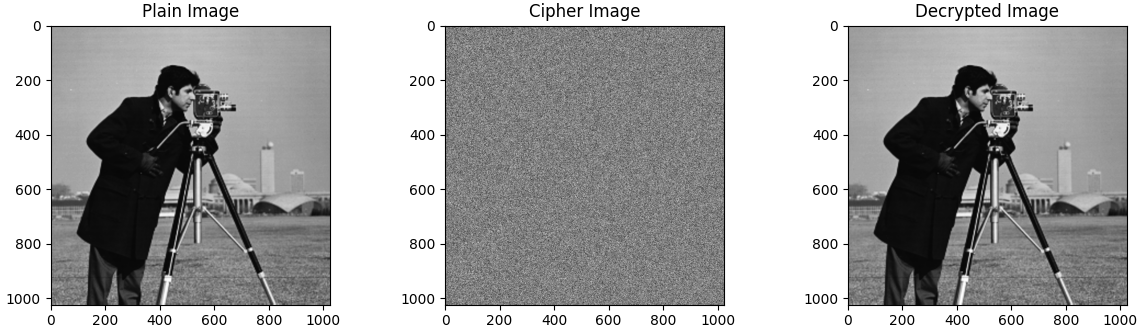
\includegraphics[width=\textwidth]{assets/result04.png}
    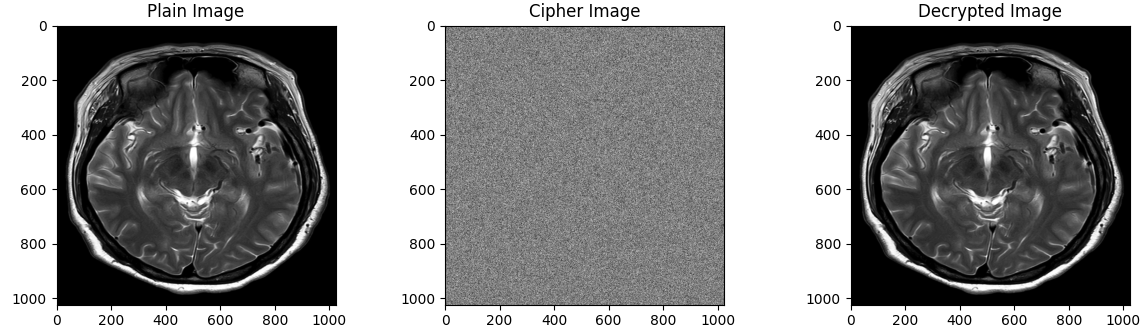
\includegraphics[width=\textwidth]{assets/result05.png}
\end{frame}

\section{تحلیل امنیت}
\subsection{مقدمه}
\begin{frame}
\makeframetitle
این بخش چندین معیار شناخته شده را توصیف می کند که معمولاً برای ارزیابی امنیت الگوریتم های جدید استفاده می شود. برای ارزیابی عملکرد و جنبه‌های امنیتی الگوریتم پیشنهادی, تحلیلی از روش پیاده‌سازی شده در زیر ارائه می‌کنیم. سرعت الگوریتم پیشنهادی نیز در آخرین بخش مورد بررسی قرار گرفته است.
از نمونه عکس \lr{Lena 512*512} استفاده خواهیم کرد
\end{frame}

\subsection{تحلیل فضای کلید}
\begin{frame}
\makeframetitle
\begin{center}
    اندازه کلید در فرآیند رمزگذاری اهمیت دارد. این کلید باید به اندازه کافی بزرگ باشد تا در برابر حملات \lr{Brute Force} مقاومت کند
کلید خصوصی توسط مقادیر 
\( a, b, c, d, e, f, g, h, x1, x2, x3, x4, x5, x6, x7, N_0 \)
 و در سیستم پر آشوب 7 بعدی ایجاد می‌شود.
  اگر دقت تخمین مقدار اولیه را برابر با 
\( 10^{16} \)
  در نظر بگیریم, بنابراین کل کلید خصوصی 
\( N_0 \times 10^{240} \)
  است که به اندازه کافی بزرگ است تا در برابر حملات \lr{Brute Force} مقاومت کند.
\end{center}
\end{frame}

\subsection{حساسیت کلید}
\begin{frame}
\makeframetitle
یک روش رمزگذاری خوب طراحی شده باید نسبت به هرگونه تغییر کوچک در شرایط اولیه کلید خصوصی استفاده شده بسیار حساس باشد.
هنگامی که این کلید کمی تغییر می کند, تصویر بازیابی شده نویز و نامفهوم می شود
یکی از پارامتر های کلید را تغیر می دهیم مثلا \lr{0.0001} به آن اضافه می کنیم نتیجه به شکل زیر خواهد بود
\vfill
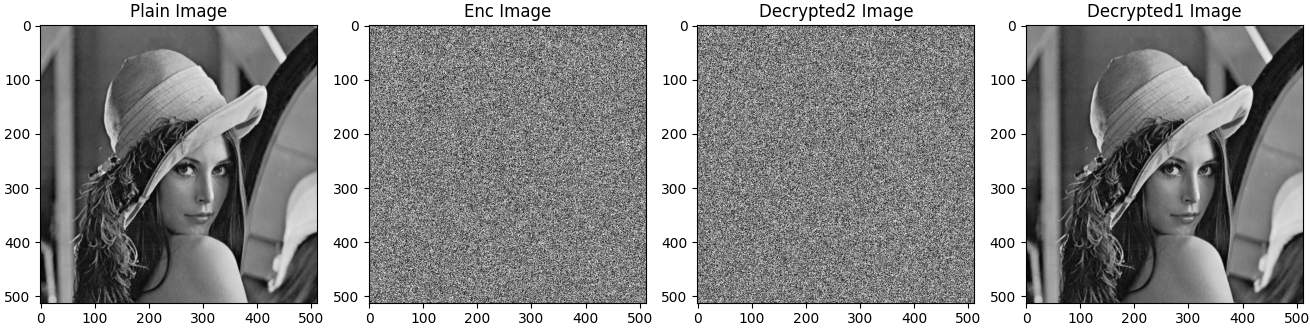
\includegraphics[width=\textwidth]{assets/result06.png}
\end{frame}

\subsection{تحلیل هیستگرام}
\begin{frame}
    \makeframetitle
    هیستوگرام یک تصویر فرکانس هر پیکسل را نشان می دهد. اگر هیستوگرام تصویر رمزگذاری شده به طور یکنواخت توزیع شود، طرح رمزنگاری می تواند به طور موثر در برابر حملات آماری مقاومت کند.
    \vfill
    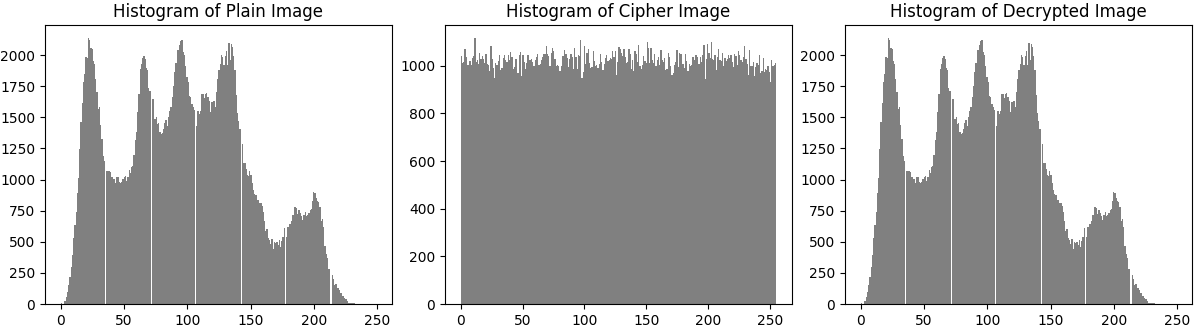
\includegraphics[width=\textwidth]{assets/result07.png}
\end{frame}

\subsection{تحلیل ضریب همبستگی}
\begin{frame}[allowframebreaks]
    \makeframetitle
    \begin{columns}
        \begin{column}{0.5\textwidth}
             یکی از مهمترین ویژگی ها در زمینه رمزگذاری تصویر، همبستگی بین هر دو پیکسل مجاور است. پیکسل ها در یک تصویر ساده دارای ضرایب همبستگی بالایی با همسایگان خود هستند. برای کاهش احتمال حملات، همبستگی بین پیکسل های همسایه یک تصویر رمزی باید بسیار نزدیک به صفر باشد. همبستگی عمودی، افقی و مورب بین هر جفت پیکسل، x و y را می توان با
        \end{column}
        \begin{column}{0.5\textwidth}
            \begin{center}
                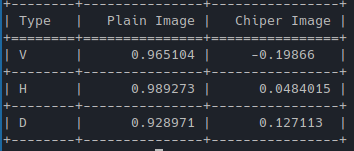
\includegraphics[width=\textwidth]{assets/result09.png}
             \end{center}
        \end{column}
    \end{columns}
    \framebreak
    \begin{align}
    \begin{split}
        R_{x,y} = \frac{cov(x,y)}{\sqrt{D(x)} \times \sqrt{D(y)}}\\
        cov(x,y) = \frac{1}{N}\sum_{i=1}^{N} (x_i - E(x))(y - E(y_i))\\
        D(x) = \frac{1}{N}\sum_{i=1}^{N} (x_i - E(x))^2\\
        E(x) = \frac{1}{N}\sum_{i=1}^{N} x_i
    \end{split}
    \end{align}
    \framebreak
    به طوری که
    و \lr{N} تعداد کل پیکسل های درگیر در محاسبات است
    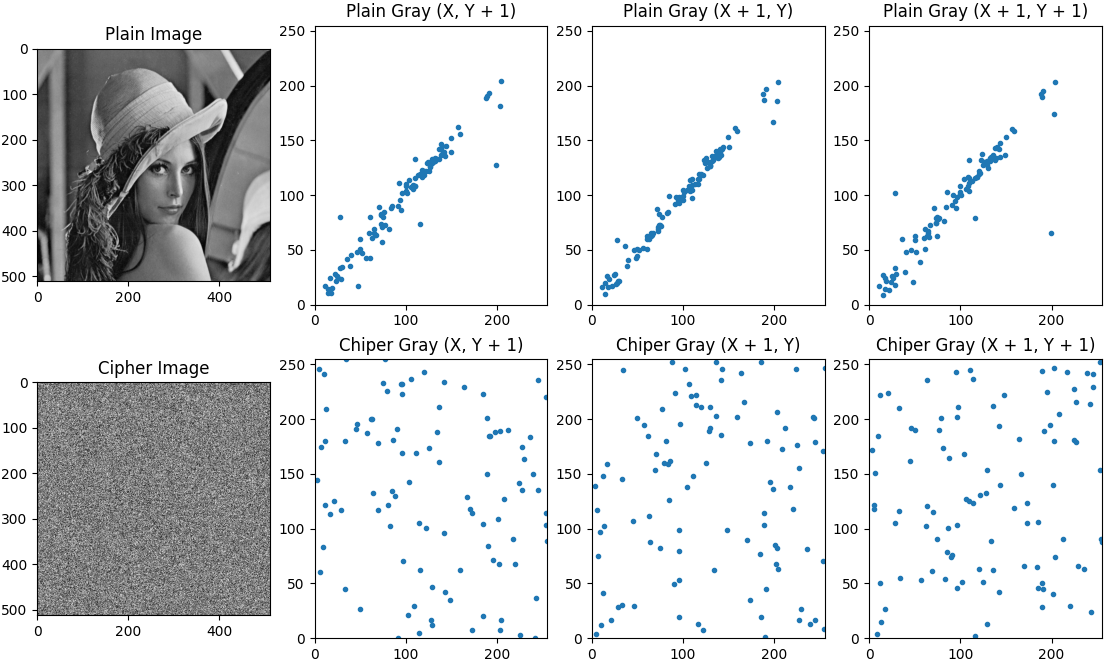
\includegraphics[width=\textwidth]{assets/result08.png}
\end{frame}

\subsection{آنتروپی اطلاعات}
\begin{frame}
    \makeframetitle
    تست آنتروپی اطاعات میزان درجه تصادفی بودن و غیر قطعی بودن در یک تصویر را اندازه گیری می کند
    \begin{align}
        H(m) = \sum_{i=1}^{2^N - 1} p(m_i) \log \frac{1}{p(m_i)}
    \end{align}
    به طوری که \lr{N} تعداد بیت های نماد \(m_i\) و \(p(m_i)\) احتمال هر کدام می باشد
    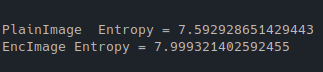
\includegraphics[width=\textwidth]{assets/result10.png}
    بهترین مقدار آنتروپی برای تصویر رمزگذاری شده 8 می باشد
\end{frame}

\subsection{تحلیل حملات دیفرانسیل}
\begin{frame}[allowframebreaks]
    \makeframetitle
    هدف از این حمله کرک کردن تصویر رمزشده   توسط ارتباط تصویر رمز شده با تصویر اصلی بدون استفاده از کلید می باشد
   برای ارزیابی این حمله از دو پارامتر \lr{UACI, NPCR} استفاده می شود
   \begin{align}
    UACI = \frac{\sum_{i=1}^{M}\sum_{j=1}^{N}|C_2(i, j) - C_1(i, j)|}{255 \times M \times N} \times 100\%\\
    NPCR = \frac{\sum_{i=1}^{M}\sum_{j=1}^{N} h(i, j)}{M \times N} \times 100\%\\
    h(i, j) = \begin{cases}
        0 & \quad \text{if } C_2(i, j) = C_1(i, j)\\
        1 & \quad \text{if } C_2(i, j) \neq C_1(i, j)
    \end{cases}
   \end{align}
   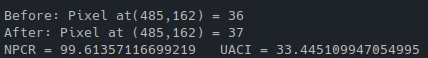
\includegraphics[width=\textwidth]{assets/result11.png}
   برای اطمینان از امنیت الگوریتم، مقدار \lr{UACI} الگوریتم های رمزنگاری تصویر باید بزرگتر از \lr{0.33} و مقدار \lr{NPCR} باید بیشتر از \lr{0.99} باشد.
\end{frame}

\subsection{حمله نویز فلفل نمکی}
\begin{frame}[allowframebreaks]
    \makeframetitle
    \vfill
    تفاوت بین تصویر اصلی و تصویر رمزگذاری شده با استفاده از نسبت سیگنال به نویز پیک (PSNR) اندازه گیری می شود. می توان آن را محاسبه کرد
    \begin{align}
        PSNR = 10 \log\left( \frac{max^2}{MSE} \right)\\
        MSE = \frac{1}{M \times N}\sum_{i=1}^{M}\sum_{j=1}^{N}(O(i, j)  D(i, j))^2
    \end{align}
    \vfill
    \framebreak
    تصاویر رمزگذاری شده هنگام انتقال از طریق کانال های ارتباطی فیزیکی مستعد نویز یا تداخل هستند.
    تکنیک رمزگذاری رمزی باید به اندازه کافی انعطاف پذیر باشد تا بتواند تصاویر رمز شده را با وجود انباشته شدن نویز رمزگشایی کند.
    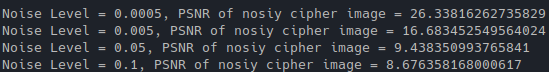
\includegraphics[width=\textwidth]{assets/result13.png}
    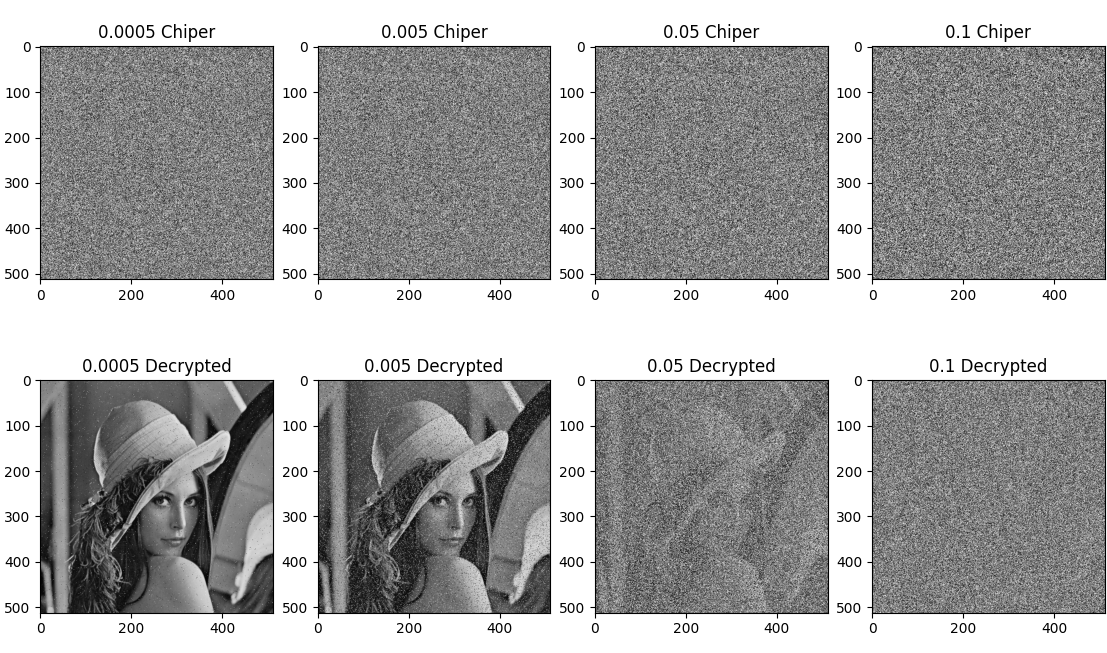
\includegraphics[width=\textwidth]{assets/result12.png}
\end{frame}

\subsection{حمله برش تصویر}
\begin{frame}
    \makeframetitle
    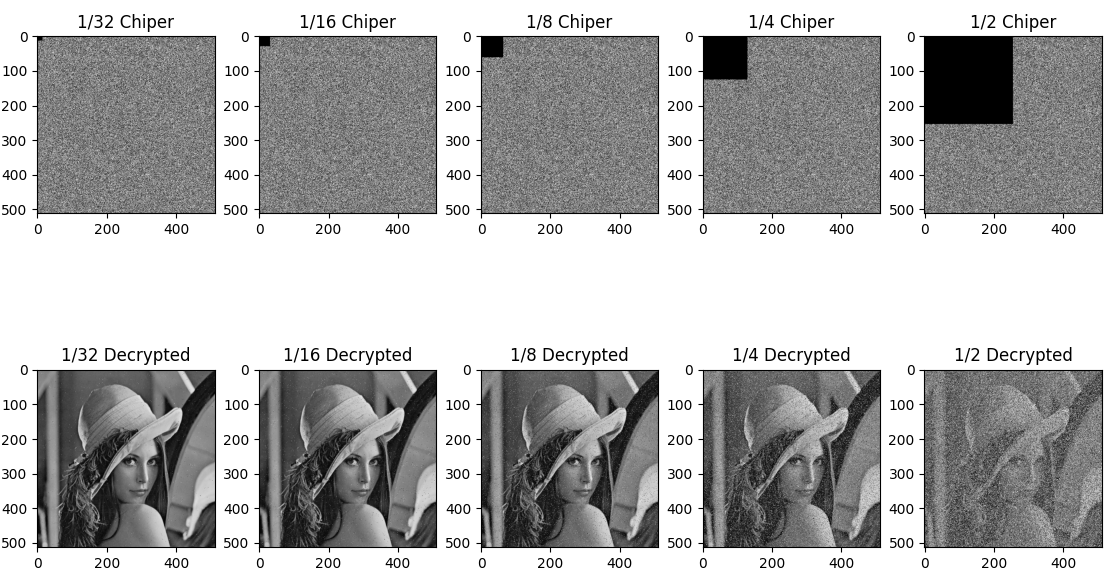
\includegraphics[width=\textwidth]{assets/result14.png}
\end{frame}

\subsection{تست سرعت}
\begin{frame}
    \makeframetitle
    هنگام توسعه یک روش رمزگذاری تصویر قوی، سرعت اجرا به همان اندازه نگرانی های امنیتی بسیار مهم است.
    \begin{latin}
        \begin{center}
            \begin{tabular}{|c|c|c|c|}
                \hline
                 Images & Size & Encryption Time & Decryption Time \\
                \hline
                Lena & \(512\times 512\) & 2.5423987944sec & 2.725500211sec\\
                \hline
                Cameraman & \(1024\times 1024\) & 10.9839755196sec & 8.5778788464sec\\
                \hline
                Tank & \(256\times 256\) & 1.3027955124sec & 1.5723612726sec\\
                \hline
                Boat & \(512\times 512\) & 2.6061833132sec & 2.4872887996sec\\
                \hline
            \end{tabular}
        \end{center}
    \end{latin}
\end{frame}

\section{نتیجه گیری}
\begin{frame}
    \frametitle{\insertsection}
    در این کار، ما یک تکنیک جدید رمزگذاری تصویر در مقیاس خاکستری را پیشنهاد کردیم. ماتریس پاسکال از مرتبه 4 با یک سیستم پر آشوب هفت بعدی در این تکنیک ترکیب شده است.
    ما در ابتدا از یک سیستم پر آشوب هفت بعدی برای تولید توالی های تصادفی استفاده کردیم و سپس سه تا از این توالی ها را برای تغییر موقعیت پیکسل انتخاب کردیم. تصویر منتشر شده در مقیاس خاکستری به مجموعه ای از 4 بلوک فرعی تقسیم می شود و ماتریس پاسکال برای تغییر مقادیر پیکسل ها برای هر بلوک فرعی استفاده می شود.
    برای تقویت امنیت، دو بار فرآیندهای سردرگمی و انتشار اجرا می شوند


\end{frame}

\section{مراجع}
\begin{frame}
    \frametitle{\insertsection}
    \begin{latin}
Ammar Ali Neamah, Journal of King Saud University - Computer and Information SciencesVolume 35 Issue 3 Mar 2023 pp 238–248 \url{https://doi.org/10.1016/j.jksuci.2023.02.014}\\
        Alghamdi, Y., Munir, A., Ahmad, J., 2022. A Lightweight Image Encryption Algorithm
Based on Chaotic Map and Random Substitution. Entropy 24 (10), 1344. \url{https://
doi.org/10.3390/e24101344.}
    \end{latin}
\end{frame}

\end{document}

